\section{Introduction}
\label{sec:intro}

\subsection{GNSS spoofing and its detection}

A Global Navigation Satellite System (GNSS) supplies a receiver with its position, its
velocity and its time. Power grids use that time to synchronise, financial systems use it
to stamp transactions, and aircraft and autonomous platforms use the position to navigate
\citep{kaplan2005understanding}. The civil signal that carries this service is public and
unencrypted, and its structure is fully specified in open documents, so a transmitter of
modest cost can generate a waveform with the same modulation, the same spreading code and
the same message format as a genuine satellite. A spoofer is such a transmitter. It emits
counterfeit satellite signals with the intention that a victim receiver tracks them in
preference to the authentic ones and reports a position or a time of the spoofer's
choosing. The threat is not hypothetical: a spoofer has steered a yacht off its intended
course through the ship's navigation system \citep{bhatti2017hostile}, and a spoofer has
captured an airborne platform in flight \citep{kerns2014uav}.

Spoofing differs from jamming in a way that determines how it must be handled. A jammer
denies the service, and the receiver observes that it has lost lock. A spoofer leaves the
receiver operating nominally while the solution it reports is wrong, so the receiver holds
no internal evidence that anything has occurred and the attack must be identified while it
is in progress \citep{psiaki2016gnss}. Capturing a receiver that is already tracking
authentic signals is correspondingly more demanding than simply transmitting at higher
power. The published procedure proceeds in three stages: the counterfeit is first aligned
with the authentic signal in code phase, carrier phase and Doppler frequency, so that the
victim's correlator sees a single undistorted peak; its power is then raised slightly above
the authentic power, typically by a few decibels; and only then is the counterfeit dragged
away from the authentic signal, carrying the tracking loops with it and moving the reported
position or time \citep{psiaki2016gnss,kerns2014uav}. A counterfeit that omits the
alignment stage does not capture the receiver at all, and acts only as interference. The
consequence is that the attacker's freedom is bounded: not every combination of transmitter
settings takes over a receiver, and an evaluation that ignores this distinction credits a
detector for rejecting transmissions that would never have succeeded.

Classical anti-spoofing tests monitor quantities the receiver computes in the course of
tracking a satellite. Representative examples are the carrier-to-noise density ratio, which
reflects received signal strength; the shape of the correlation function, which distorts
when a second copy of the same code is present; and the agreement between code and carrier
measurements of a single satellite \citep{akos2012gnss,psiaki2016gnss}. Each such test
identifies one physical signature of an attack, which makes it interpretable and also makes
it evadable: a spoofer that holds the named quantity within its nominal range passes the
test, and the set of tests a receiver runs is public knowledge.

\subsection{Learned detectors and how they are evaluated}

The limitation of signature based tests has motivated detectors inferred from data. A
machine learning detector is a classifier trained on labelled epochs, some recorded while
the receiver tracked authentic signals and some recorded under spoofing, which learns which
joint configurations of receiver measurements indicate an attack. Because such a classifier
reads many measurements simultaneously, it can exploit dependencies that no single hand
written statistic encodes, and recent work reports high detection accuracy for both deep
architectures and classical classifiers applied to receiver observables
\citep{borhanidarian2024deep,li2025realtime,chen2025cgan}. Physics constrained networks
extend the approach towards attacks absent from the training data by imposing relations that
authentic signals must satisfy \citep{song2026generalized}.

The evaluation practice that accompanies this literature is uniform: a detector is scored
against a fixed collection of recorded or simulated attacks. Those attacks were selected
before the detector existed, by whoever assembled the corpus, and they do not respond to the
classifier under test. A spoofer does respond. It selects the counterfeit power, the rate at
which it drags the code away from the authentic code, and the frequency and phase of its
carrier, and each of those choices alters the measurements the victim receiver produces and
therefore alters what the detector reads. Detection accuracy obtained against a fixed corpus
describes the corpus. It does not, by itself, characterise behaviour against an adversary
that chooses what to transmit, and the two quantities need not coincide.

\subsection{Receiver in the loop evaluation of transmitted attacks}

This paper evaluates fourteen detectors under attacks that are radio signals and not
perturbations of a measurement table. A counterfeit GPS L1 C/A waveform is synthesised at
sample level, summed with authentic recorded samples from the Texas Spoofing Test Battery
\citep{humphreys2012texbat,humphreys2016texbatds78}, passed through a model of the receiver
front end, and tracked by the FGI-GSRx software receiver \citep{fgigsrx}, published by the
Finnish Geospatial Research Institute (FGI). The observables
each detector reads are those the receiver computes while tracking that sum.
Figure~\ref{fig:geometry} contrasts authentic operation with a spoofing attack, and
Figure~\ref{fig:pipeline} shows the evaluation chain.

% Figure source: figures_src/static/fig_spoofing_geometry.png (hand made)
\begin{figure*}[t]
\centering
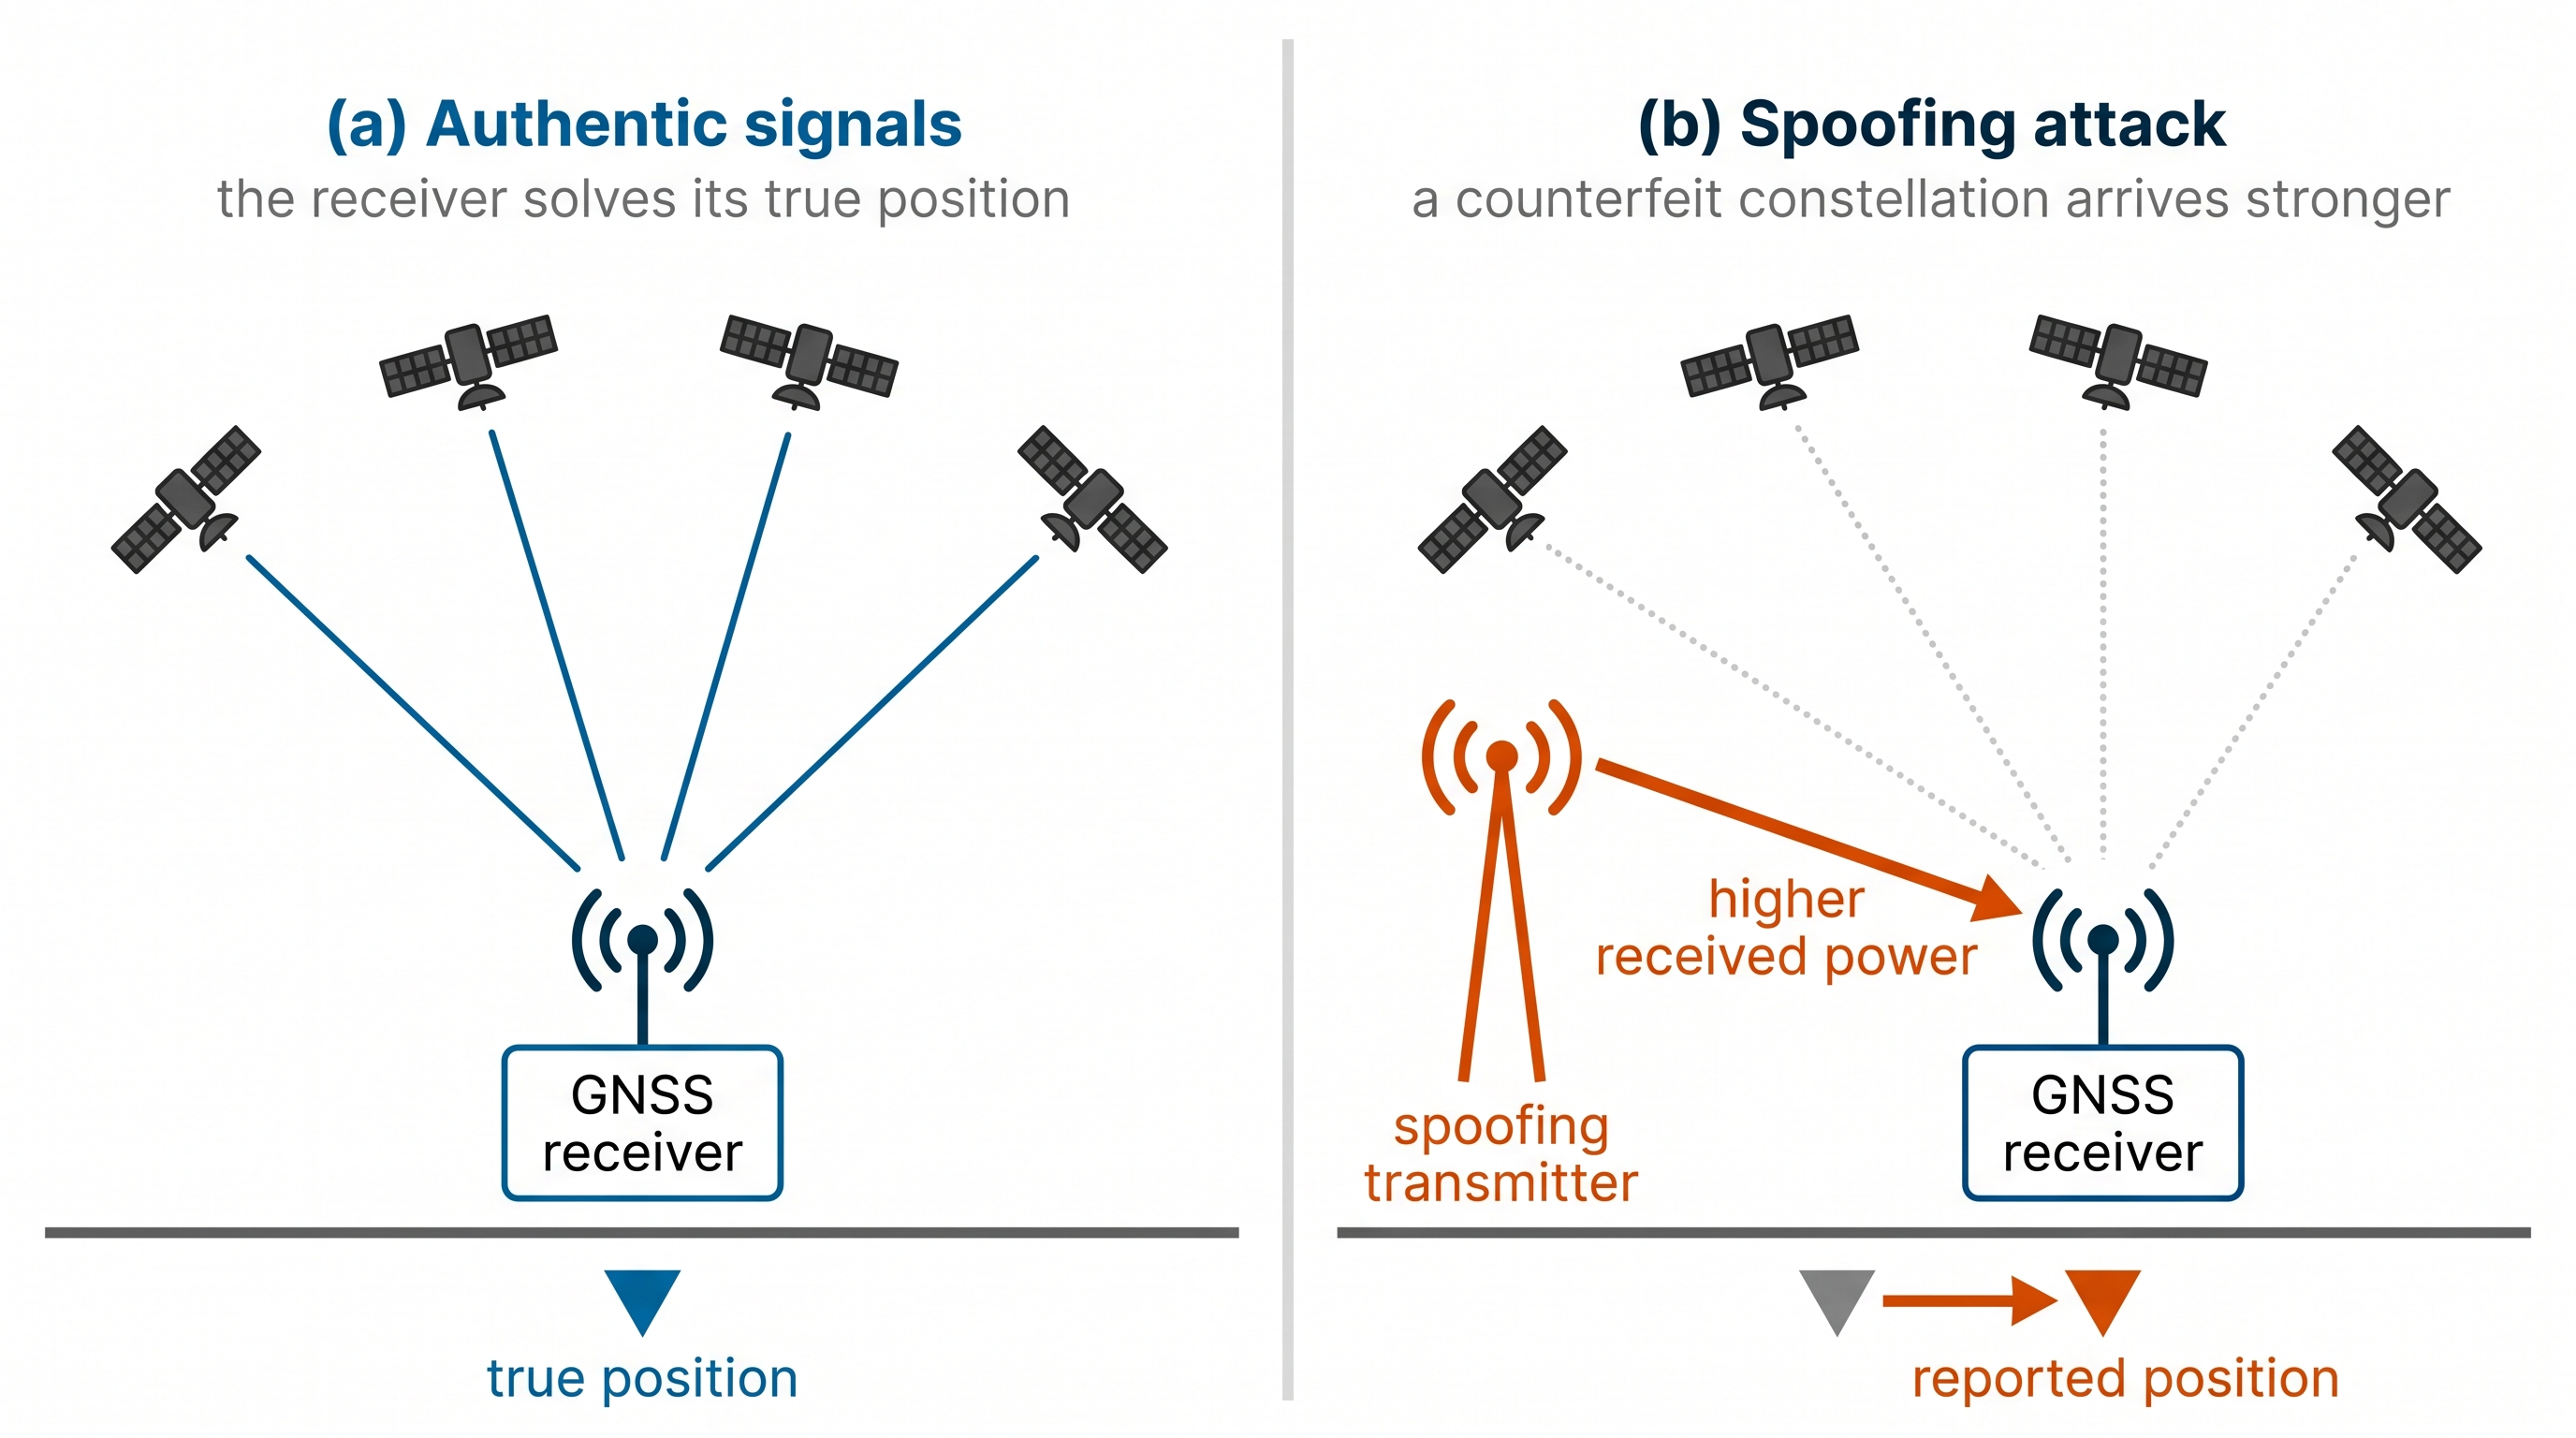
\includegraphics[width=\textwidth]{figures/fig_spoofing_geometry.png}
\caption{A GNSS receiver under authentic signals and under a spoofing attack. In (a) the receiver solves its true position from the satellite signals. In (b) a spoofing transmitter emits a counterfeit constellation that arrives at higher received power, captures the tracking loops, and moves the reported position while the receiver continues to report a valid solution.}
\label{fig:geometry}
\end{figure*}

% Figure source: figures_src/static/fig01_pipeline (hand made, distributed by
% figures_src/sync.py). Do not edit the copy inside figures/, it is overwritten.
\begin{figure*}[t]
\centering
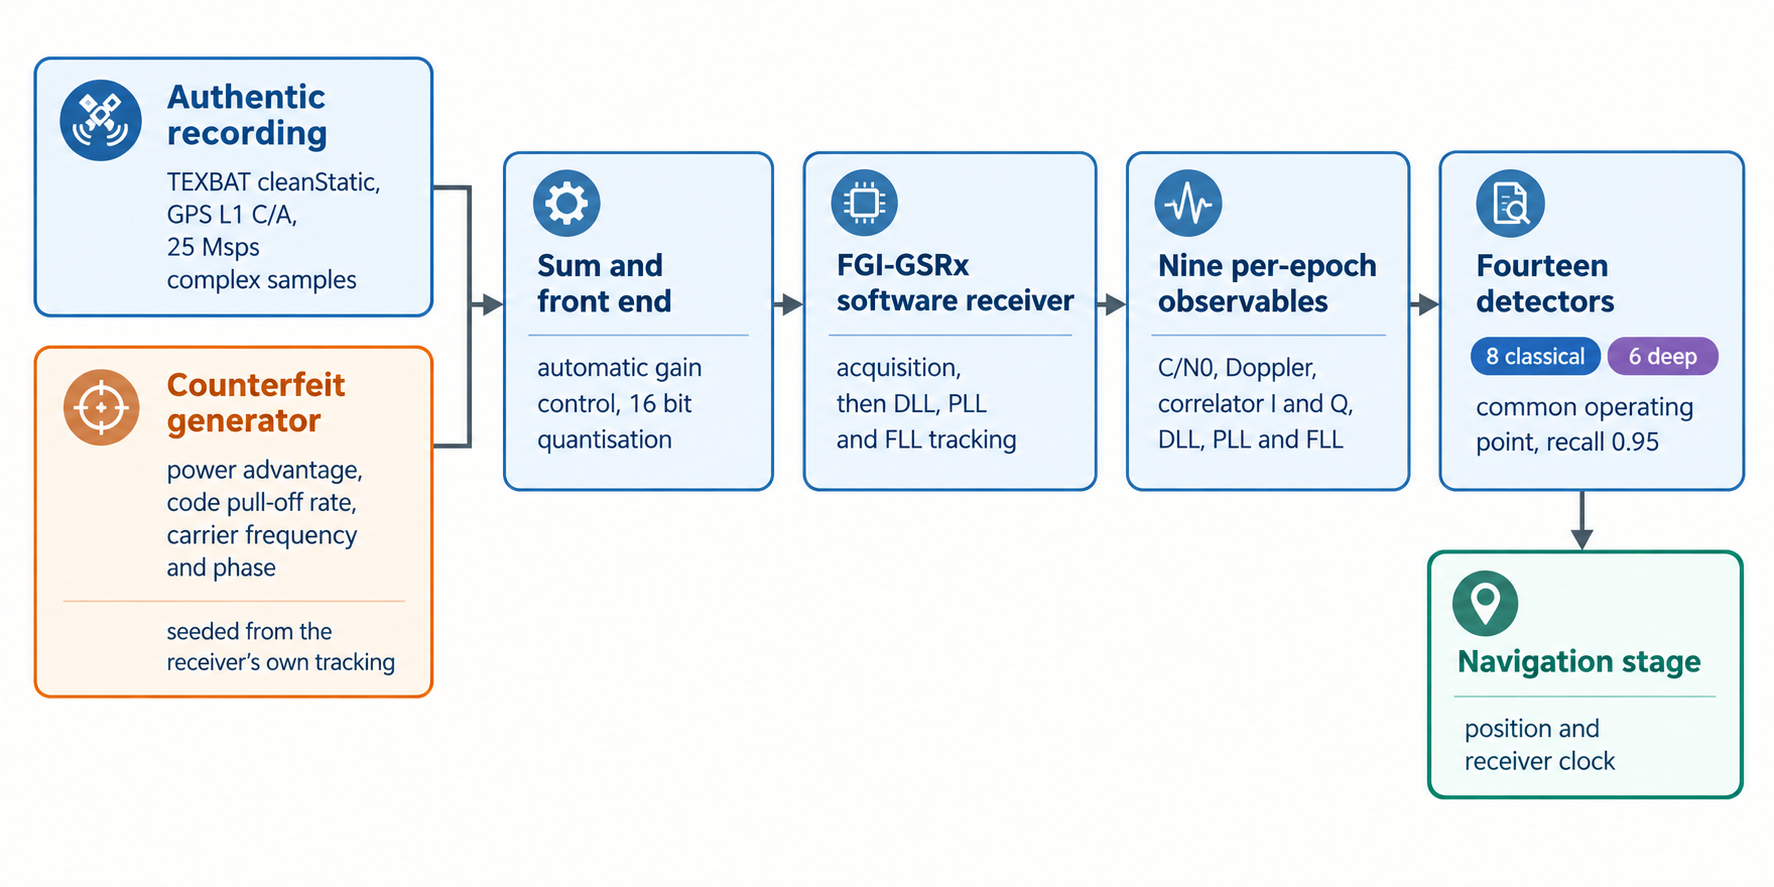
\includegraphics[width=\textwidth]{figures/fig01_pipeline.jpeg}
\caption{How a transmitted attack becomes a detector input. A counterfeit GPS L1 C/A
signal is generated as radio samples and added to authentic recorded samples. The sum
passes through the front end and is tracked by the FGI-GSRx software receiver, which
produces the nine per-epoch measurements the detectors read. The same tracking output
also feeds the navigation stage, which yields the position and the receiver clock.}
\label{fig:pipeline}
\end{figure*}

Evaluating at the waveform level fixes the relationship between the adversary's actions and
the detector's inputs, for the regime this study addresses. The generator is seeded from the
receiver's own tracking of the authentic recording, so the counterfeit arrives aligned, and
the evaluation therefore characterises detector behaviour conditional on an adversary having
achieved that alignment. Achieving it is a separate problem, and the results here should be
read as conditional on capture and not as an end to end demonstration. The adversary acts on transmitter settings, listed in
Table~\ref{tab:attacker}, which are the quantities a physical spoofer controls; the
observables follow from a receiver tracking the resulting signal, and inherit whatever
dependencies receiver processing imposes on them. Several of the observables a detector
reads are computed from the same underlying correlator output and therefore cannot be varied
independently, so the mapping from adversary action to detector input is not the identity
and is not free. The generator is validated against data set ds7 of the battery, a recorded
attack whose construction is documented in full \citep{humphreys2016texbatds78}, and
reproduces the observables recorded for it.

All fourteen detectors are placed at a common operating point, defined as the highest
decision threshold at which a detector still flags 95 percent of spoofed samples on clean
validation data. A common operating point is necessary because a classifier's error rates
move together with its threshold, so detectors read at different thresholds are not
comparable. The false alarm rate each detector pays to meet the recall floor is reported
alongside every result.

Three findings follow. First, ranking on clean data inverts under transmitted attack: the
random forest attains the highest clean $F_1$ score, the harmonic mean of precision and
recall, and the lowest false alarm rate, yet fails to flag 55 of the 126 transmitted attacks
that capture the receiver, flagging as few as 0.1 percent of the spoofed samples of one of
them. Second, the detectors that flag every attack achieve this only by flagging 46 to 74
percent of authentic data, a regime in which a receiver would alarm almost continuously, so
their apparent resistance is not operationally available. Across all fourteen, false alarm
rates at this operating point span 34 to 96 percent. Third, a missed attack propagates to
the navigation solution: followed through the navigation stage, one such attack drives the
receiver clock at 48.89 nanoseconds per second against a commanded 48.87, after the
receiver's own drift of 0.12 nanoseconds per second has been measured and removed.

\subsection{Contributions}

The principal contribution is the evaluation methodology, because the findings that
follow hold only if the detector inputs are produced by receiver processing of a
signal an adversary could transmit. The remaining four rest on it: the second supplies
the adversary's choice set, the third and fourth measure what existing detectors do
against that choice set and what a failure costs, and the fifth relates the result to
the feature space evaluation the literature more commonly reports.

\begin{enumerate}
  \item \textbf{An evaluation methodology in which every attack is a transmitted
  waveform.} Each attack is synthesised as radio samples, summed with authentic
  recordings and tracked by a software receiver, so that the detector inputs are
  produced by receiver processing of a transmittable waveform. The generator is
  validated by reproducing a recorded attack whose construction is published.

  \item \textbf{A library of transmitted attacks.} Two hundred and nine transmitter
  settings spanning counterfeit power, code pull-off rate and carrier alignment, of
  which 126 satisfy the published conditions for receiver takeover. The library
  expresses the adversary's choice set as data and separates transmissions that
  capture a receiver from those that do not.

  \item \textbf{A comparative evaluation of fourteen detectors,} eight classical and
  six deep, against that library at a common operating point, reporting for each
  detector the number of transmitted attacks it fails to flag together with the false
  alarm rate it incurs on authentic data, with exact binomial intervals on every
  count.

  \item \textbf{A navigation domain measurement} establishing that a missed attack
  reaches the position and timing solution, obtained by propagating one such attack
  through the navigation stage and comparing the induced clock drift against the rate
  the transmitter was configured to impose.

  \item \textbf{A comparison against feature space evaluation,} in which the same
  detectors are attacked by perturbing measurements directly. The two views agree on
  which detectors are fragile, and disagree on the support vector machine, whose
  apparent resistance is accounted for by its false alarm rate. A perturbation size
  reported without that rate would invert the conclusion.
\end{enumerate}

\subsection{Organisation}

Section~\ref{sec:related} reviews spoofing detection and the robustness of learned
classifiers. Section~\ref{sec:signal} describes the receiver processing chain and the
observables it produces. Section~\ref{sec:threat} defines the threat model and the attack
space. Section~\ref{sec:method} presents the waveform generator, its validation, the attack
library, the detector set and the operating point calibration.
Section~\ref{sec:results} reports the results, Section~\ref{sec:discussion} examines their
implications for receiver integrity and states the scope of the study, and
Section~\ref{sec:conclusion} concludes.
